\scanpage{124}
% archive foliation: 123
\uline{Cas car. 2 ou 3} --- Ici il faut supposer
\[ B=A[T]/(T^{p^2}-\alpha), \]
sinon l'énoncé (modulo rectification de la \deleted{définition}\inserted{description} des $D_t^{(i)}\ldots$) du résultat sur \unsure{formes d'hog. comme}, et la réduction au cas $\alpha=0$, $s\equiv t\ (t^3B)$, est comme dessus. Il faut prouver que $s=t$, donc si
\[s=t+at^d\qquad(3\leq d\leq\deleted{\unsure{p}}p^2-1)\]
alors $a=0$. On trouve comme tantôt
\[a\binom d3=0\quad\text{i.e.}\quad a\underbrace{c_{3,d-3}}_{\text{coeff. binom.}}=0,\]
d'autre part $c_{\unsure{2|3},d-3}\in\mathbb F_p^*$ ssi. \deleted{$d\text{ et }d-3$} pour
\[
\begin{gathered}
d-3=d_0+d_1p\\
\unsure{3}=d'_0+d'_1p
\end{gathered}
\qquad(0\leq d_0,d_1,d'_0,d'_1\leq p-1)
\]
on a $d_0+d'_0\leq p-1$, $d_1+d'_1\leq p-1$.

1) Cas car. $p=2$, \deleted{$\unsure{d-d'_0}=\unsure{1}(d_0-1)+(d_1-1)p$}
\deleted{Car $d_0,d_1\geq1$ \unsure{le cas favorable est celui}.}
Car l'\uline{unique} est $d=3$ \deleted{$\unsure{d\leq p}$}.
\deleted{\unsure{donc}}
\[c_{3,0}=1\quad\Longrightarrow a=0\qquad\text{OK}\]
\deleted{$\unsure{d_0=d_1=0}$}

2) \uline{Cas $p=3$}. \deleted{\unsure{pour}}
\deleted{Si $d_1\ne0$ i.e. $d_1\geq1$,
\[
d-3=d-p=d_0+(d_1-1)p,\quad\text{et}
\]
\[
c_{d,d-3}=c_{d_0,d_0}c_{d_1,d_1-1}\quad\text{dans }\mathbb F_p
\]
\[
\in\mathbb F_p^*\quad\text{ssi}\quad
\begin{gathered}2d_0\leq p-1=2.\\2d_1-1\leq p-1=2.\end{gathered}
\]
i.e. $d_1=1$, $d_0=0$ ou $1$, donc cas qui échappent
\[
\text{c) }\textcircled{$d_1=0$},\quad\text{a) }d_1=2.\qquad\text{b) }d_1=1,\ d_0=2.
\]
\unsure{Le cas} $d_1=0$ est au fond favorable, car alors $3\leq d\leq p-1$ donc $c_{d,d-3}$}

\[
d-3=d_0+d_1p\qquad0\leq d_0,d_1\leq2
\]
\margin{et comme $0\leq d-3\leq5$ (car \deleted{$d$} $3\leq d\leq p^2-1=8$)}
\deleted{$0\leq d_1\leq\unsure{3}$}
\[\inserted{d_1\leq1}\]
\[3=0+1\times p\]
La condition $c_{3,d-3}\in\mathbb F_p^*$ signifie ici
\[
d_1+1\leq p-1\quad\text{i.e.}\quad\deleted{\unsure{p}}\ d_1+1\leq2\quad\text{i.e.}\quad d_1\leq1,
\]
qui est vérifiée. On gagne encore !
\figure{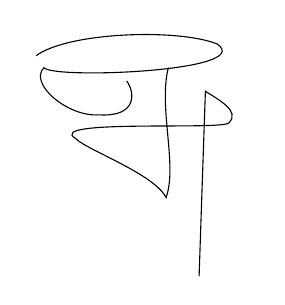
\begin{tikzpicture}[x=1cm,y=1cm]
\draw (0,2.8) .. controls (0.4,3.1) and (1.8,3.15) .. (2.3,2.95) .. controls (2.8,2.6) and (0.2,2.5) .. (0.1,2.65) .. controls (-0.1,2.45) and (0.4,2.02) .. (0.8,2.05) .. controls (1.3,2.02) and (1.25,2.35) .. (1.15,2.48);
\draw (1.68,2.65) .. controls (1.55,2.15) and (1.8,1.4) .. (1.65,1.0) .. controls (1.5,1.3) and (0.65,1.6) .. (0.5,1.75) .. controls (0.1,2.0) and (2.4,1.85) .. (2.45,1.95) .. controls (2.6,2.1) and (2.3,2.25) .. (2.15,2.35) -- (2.07,0);
\end{tikzpicture}}
